\documentclass[11pt]{amsart}
\usepackage{geometry}                % See geometry.pdf to learn the layout options. There are lots.
\geometry{letterpaper}                   % ... or a4paper or a5paper or ... 
%\geometry{landscape}                % Activate for for rotated page geometry
%\usepackage[parfill]{parskip}    % Activate to begin paragraphs with an empty line rather than an indent
\usepackage{graphicx}
\usepackage{amssymb}
\usepackage{epstopdf}
\DeclareGraphicsRule{.tif}{png}{.png}{`convert #1 `dirname #1`/`basename #1 .tif`.png}

\newtheorem{Def}{Definition} %[section]
\newtheorem{Example}[Def]{Example}
\newtheorem{Prop}[Def]{Property}
\newtheorem{Lemma}[Def]{Lemma}
\newtheorem{Thm}[Def]{Theorem}
\newtheorem{Conj}[Def]{Conjecture}
\newtheorem{Cor}[Def]{Corollary}

\newcommand\bpf[1][]{\smallskip\noindent{\bf Proof#1.}\quad}
\newcommand\epf{\qed\medskip}
\newcommand{\up}[1]{\ensuremath{^{\textrm{#1}}}}

\newcommand\N{\mathbb N}

\title{Brief Article}
\author{The Author}
%\date{}                                           % Activate to display a given date or no date

\begin{document}

{\bf Ideas While Learning Set Theory}

These notes are not meant to be considered an academic paper,
or anything close to that. They are a collection of my personal
thoughts while learning set theory.

\section{Equivalences}

This section describes some explicitly constructed, somewhat natural 1-1 correspondences between
some collections of objects, such as sets, multi sets, lists, trees, and $\N$.

\subsection{Numbers $\leftrightarrow$ binary trees}

Choose any 1-1 correspondence $f : \N_{\ge 1} \to \N^2_{\ge 0}$.
I like to think of such a map as a counting of grid points in an array, such as this:

$$
\begin{array}{c|cccc}
 & 0 & 1 & 2 & 3 \\
 \hline
 0 & 1 & 2 & 4 & 7 \\
 1 & 3 & 5 & 8 \\
 2 & 6 & 9 \\
 3 & 10 &&& \ddots \\
\end{array}
$$

That's what Hausdorff calls ``the diagonal array.''
It's pretty easy to compute both ways.

Once you have $f = (f_1, f_2)$, then you build a binary
tree from a number $n$ recursively like this:

If $n=0$, then it's the empty tree (no root).
Otherwise, give it the left child $f_1(n)$ and
right child $f_2(n)$, keeping in mind that if
either has value 0, this means no child in that direction.
If you don't want to count the no-root tree, then start
counting at $n=1$ instead of $n=0$.

\subsection{Numbers $\leftrightarrow$ ordered $n-$ary trees}

An ordered $n-$ary tree is the natural extension of binary trees.
To be clear, binary trees are used (in my experience) most often
in a computer science context, where the left and right subtrees
are always distinguished - i.e., they are ordered. This is a bit
different from the typical math tree, where there is no intrinsic order.

The mapping is exactly the same as the binary case, except that
we must choose a 1-1 correspondence $g: \N_{\ge 1} \to \N^n_{\ge 0}$;
then the $k^\text{th}$ child of a tree numbered by $m$ will be
numbered by $g_k(m)$, where $g_k(m)$ is the  $k^\text{th}$ coordinate
of $g(m)$.

\section{Total Orders}

\subsection{A fixed-point theorem for total orders}

The following result was motivated originally by the
Banach fixed-point theorem. After proving it, I found out
about the Bourbaki-Witt (B-W) theorem, which is extremely similar,
and probably only this theorem or B-W is needed (i.e. one can be
derived easily from the other), although I haven't figured out which yet.

The notation $\sup (A)$ means $\min \{x : x \ge a \forall a \in A\}$,
which does not exist for every set $A$.

\begin{Thm}
Suppose that $X$ is totally ordered, that $\sup (A)$ exists
$\forall \text{ nonempty } A\subset X$ with an upper bound,
and that $f:X\to X$ is an
order-preserving map with $x_0 < f(x_0)$ and $f(x_1) < x_1$,
for $x_0 < x_1$. Then $\exists y \in (x_0, x_1)$ with $f(y) = y$.
\end{Thm}

\bpf
Define
$$ A = \{ y \in [x_0, x_1] : x_0 \le z \le y \implies f(z) > z \}. $$
Intuitively, $A$ is the largest convex set with left endpoint $x_0$
where $f(a) > a \forall a \in A$.

% insert set_theory_ideas1.pdf here

\centerline{
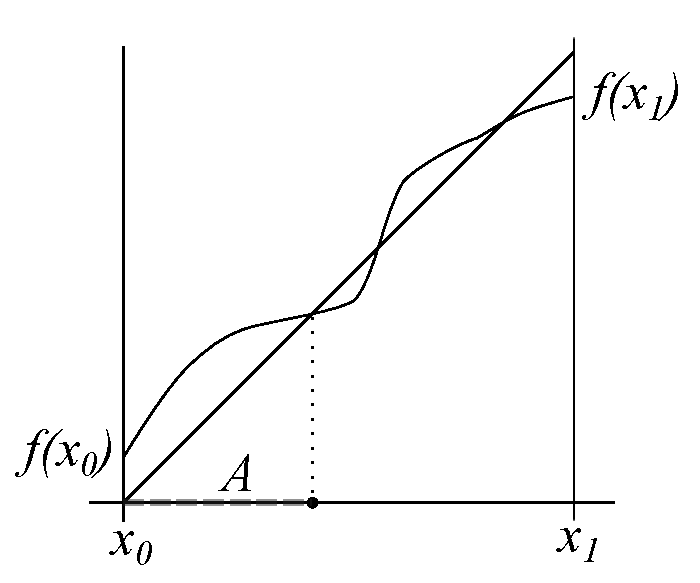
\includegraphics[width=6.0cm]{set_theory_ideas1.pdf}
}

Let $\beta = \sup (A)$, which exists since $A$ is nonempty,
having $x_0 \in A$, and has an upper bound, $x_1$.

If $\gamma = f(\beta) < \beta$, then $\gamma \in A$, but
$$ \gamma < \beta \implies f(\gamma) < f(\beta)
  \implies f(\gamma) < \gamma, $$
%$f(\gamma) = f(f(\beta)) < f(\beta) = \gamma$,
which contradicts
$f(\gamma) > \gamma$ for everything in $A$.
So $f(\beta) \ge \beta$. If $f(\beta) = \beta$, we're done,
so assume $f(\beta) > \beta$.

Suppose $w \in [x_0, x_1]$.

If $\beta < w$ and $\big(f(b) > b \,\forall\, b \in (\beta, w]\big)$,
then $w \in A$, which would contradict $w > \beta \ge A$.
So $\exists\, b_0$ with $\beta < b_0 \le w$
and $f(b_0) \le b_0$.  Then $f(\beta) < f(b_0) \le b_0 \le w$.

At this point we have both
$$ \beta < w \implies f(\beta) < w $$
and
$$ \beta > w \implies w \in A \implies f(\beta) > f(w) > w.$$

So $f(\beta) \in [x_0, x_1] \setminus \{ < \beta \} \setminus \{ > \beta \} = \{\beta\}$.
\epf

Note that $\sup (A)$ need only  exist for the specific set $A$
used in the proof, so that part of the theorem's conditions could be relaxed.

\subsection{Matching well orders}

This is an old idea for me, but I wanted to record it in this section.

First, we need a lemma from Jech's {\em Set Theory} (I have the 3\up{rd} edition).

\begin{Lemma}\label{b_squared_is_b_lemma}
Suppose infinite ordinal $\omega_a$ is the first  of its cardinality -- that is, $|\omega_b| < |\omega_a|$
for all $\omega_b < \omega_a$.
Also suppose that well-ordered set $A$ is of order type $\omega_a$. Then any
proper subset $B \subsetneq A$ has $|B|^2 = |B| < |A|$.
\end{Lemma}

The fact that $A$ can be well-ordered as $\omega_a$ is not necessarily true without
the axiom of choice (not obvious), and in fact someone (I think Tarski) has proven that
if $|A|^2=|A|$ for all infinite sets $A$, then the axiom of choice must hold.

(Asaf Karagila helped me out a bit here via math.stackexchange.com.)

Theorem 3.5 in Jech has a proof which also proves this lemma.

There is an interesting perspective on this lemma which I particularly like:

\begin{Lemma}
Suppose infinite ordinal $\omega_a$ is the first  of its cardinality, and its
cardinality is not the limit of $|\omega_b|$ for $\omega_b < \omega_a$.
Then any increasing ordinal sequence $\left< \eta_i | i \in \omega_b \right>$
with $\eta_i, \omega_b < \omega_a$ must have $\lim_i \eta_i < \omega_a$.
\end{Lemma}

The lemma follows because all the $\eta_i$ must have $|\eta_i| \le \mathfrak b$,
where $\mathfrak b$ is the largest cardinal in $\omega_a$ (which means
$\mathfrak b < |\omega_a|$).
We also know that $|\omega_b| \le \mathfrak b$,
and by the previous lemma, that $\mathfrak b^2 = \mathfrak b$. So
$$ | \lim \eta_i | = | \cup_{i\in\omega_b} \eta_i | \le \mathfrak b^2 = \mathfrak b < |\omega_a|.$$

I'd summarize that last lemma as ``you can't sneak up on successor ordinals.''

Here's the result these lemmas are used for:

\begin{Thm}[Matching Well Orders]
Suppose infinite set $X$ is well ordered by both $\le_1$ and $\le_2$.
Then there is a subset $Y \subset X$ with $|Y| = |X|$ on which
$\le_1$ and $\le_2$ agree; the axiom of choice is not needed.
\end{Thm}

The proof in the general form looks a bit unintuitive, so first I'll mention the
main idea by looking at a special case with $X=\N$.
Suppose I have two orders $\le_1$ and $\le_2$ such that
$\N$ under $\le_i$ has order type $\omega$ for both $i=1,2$.

For each integer $n$, we'll inductively build a subset of $\N$ on which
these orders agree. For the base case, we can just use the $\le_1$-min
element.

Suppose we have set $S\subset\N$ on which the orders agree.
The next element $e$ that we append must have both $S <_1 e$ and $S <_2 e$.
So we want to exclude $T = \{ m : m \le_2 s \text{ for any } s \in S\}$.
Because $\N$ under $\le_2$ has order type $\omega$, we know that each
set $\{ \le_2 s \}$ is finite; $T$ is the union of $\{ \le_2 s\}$ over $s\in S$, so that
$T$ is also finite. Thus $U = \N - S - T$ is nonempty, and we can choose the
$\le_1$-min element of $U$ as the next element to append to $S$.

By induction on the size of $S$, we get a countably infinite subset of $\N$ on which the orders agree.
I don't think it's obvious how to extend this to an arbitrary set $X$, so I'll prove that carefully.

I would summarize this special case as saying, if you have any two enumerations of $\N$, there's
an infinite subset on which they are identical.

For the proof I will also use this easy lemma:

\begin{Lemma}\label{first_ordinal_lemma}
If $X$ is well ordered by $\le$, then there is a subset $Y\subset X$ with
$|Y| = |X|$ where the order type of $Y$ under $\le$ is the first ordinal
with cardinality $|X|$.
\end{Lemma}

This lemma is true because we can look at the set $Z = \{ x\in X : |\{ < x \}| = |X| \}$.
If $Z$ is empty, then $Y=X$ satisfies the lemma. Otherwise, $Z$ has a $\le$-first element $z$,
and we can let $Y = \{ < z \}$.

\bpf
Ok, let's get this party started.

We have an infinite set $X$ that is well ordered by $\le_1$ and $\le_2$.
Let $\omega_x$ denote the first ordinal number with the cardinality of $X$.

We'll split this into two cases:

{\bf Case 1 } $|\omega_x|$ is a successor cardinal

When we say {\em successor cardinal}, we mean among
the cardinals that derive from ordinals. These cardinals are
well ordered, so they are either successors or limits, without
need for the axiom of choice. Hence our split into cases 1 and 2 ---
$|\omega_x|$ is a successor or limit cardinal --- is valid without the axiom of choice.

Use lemma \ref{first_ordinal_lemma} on both $\le_1$ and $\le_2$ (one
at a time) to get a subset $Y \subset X$
with $|Y| = |X|$ where $|\{ <_i y \}| < |X|$ for all $y\in Y$, $i=1,2$.

We will now define, via transfinite induction, a subset of $Y$ on which the orders agree.
We'll use a 1-1 function $f : \omega_x \to Y$, defining $f(\chi)$ in terms
of $f( \{ < \chi \} )$, so that the orders agree on $f( \{ \le \chi \} )$.

Suppose $f$ is already defined on the domain $\{ < \chi \}$ for some fixed $\chi \in \omega_x$.
Let $S = f( \{ < \chi \} )$, and 
let $T = \{ y \in Y : y \le_2 s \text{ for some } s \in S \}$.
This way, any element $e \in Y - T$ must have $e >_2 s$ for every $s \in S$.

Because $|\omega_x|$ is a successor cardinal, it has an immediate predecessor
$\mathfrak b$.
We chose $Y$ so that $|\{\le_2 s\}| < |Y|=|X|$, so $|\{\le_2 s\}| \le \mathfrak b$.
And $|S| = |\{ < \chi \}| < |\omega_x| = |X|$, so $|S| \le \mathfrak b$.
Then $|T| = |\cup_{s\in S}\{\le_2 s\}| \le \mathfrak b^2 = \mathfrak b < |Y|$,
so that $Y-T$ is nonempty
(the $\mathfrak b^2 = \mathfrak b$ part comes from lemma \ref{b_squared_is_b_lemma}).
Thus we can define $f(\chi )$ as the
$\le_1$-first element of $Y-T$, completing case 1.

{\bf Case 2 } $|\omega_x|$ is a limit cardinal

In this case, we can build $f_\mathfrak b$ for any ordinal-based cardinal $\mathfrak b$ below
$|\omega_x|$ using the technique from case 1. If each step results in a
superset of the previous steps, then we can take the union of the results to
get a consistent subset of $Y$ with the same cardinality.

Let's build $f_\alpha$ to have cardinality $\aleph_\alpha$.
In particular, let $\omega_\alpha$ be the first ordinal so that
$|\omega_\alpha| = \aleph_\alpha$, and we'll define
$f_\alpha$ on the domain $\omega_\alpha$.

{\bf Case 2a} $\aleph_\alpha$ is a successor cardinal

(Again the term successor cardinal in this proof means among
ordinal-based cardinals, to avoid using the axiom of choice.)

Let $\aleph_\beta$ denote the predecessor of $\aleph_\alpha$,
with $\omega_\beta$ the first ordinal of size $\aleph_\beta$.
Then $f$ has already been defined on $\omega_\beta$.

Choose $Y' \subset X$ so that $Y'$ has order type $\omega_\alpha$
under $\le_1$. Choose $Y\subset Y'$ so that $|Y| = |Y'| = \aleph_\alpha$
and $| \{ <_2 y \} | \le \aleph_\beta$ using lemma \ref{first_ordinal_lemma}.
Note that this $Y$ is a superset of any other $Y$ chosen for a smaller cardinal
as $\aleph_\alpha$.

We'll inductively define $f_\alpha$ on every $\chi \in \omega_\alpha$ with $\chi \ge \omega_\beta$.
For $\chi \in \omega_\beta$, we set $f_\alpha(\chi) = f_\beta(\chi)$.

As above, let $S = f_\alpha( \{ < \chi \} )$,
and $ T = \{ y \in Y : y \le_2 s \text{ for some } s \in S \}$; we'll verify that the size of $T$ is bounded.
We know $|S| = \aleph_\beta$ and $|\{ \le_2 s \} | \le \aleph_\beta$, so
$$ |T| = \left|\cup_{s\in S} \{ \le_2 s \}\right| \le \aleph_\beta^2 = \aleph_\beta < |Y| = \aleph_\alpha. $$

This means $Y-T$ is nonempty, and we can define $f_\alpha(\chi)$ as its $\le_1$-first element, as before.

{\bf Case 2b} $\aleph_\alpha$ is a limit cardinal

We have been careful to define $f_\alpha$ consistently on all previous sets ---
in other words, if $\chi$ is in the domain of $f_\gamma$ for any $\aleph_\gamma < \aleph_\alpha$,
then $\chi$ is in the domain of $f_\alpha$ and $f_\gamma(\chi) = f_\alpha(\chi)$.

Thinking of $f_\gamma$ as a set of ordered pairs,
we can use a union to define a limit:
$$ f_\alpha = \cup_{\aleph_\gamma < \aleph_\alpha} f_\gamma. $$

If there exists $x, y$ in the range of $f_\alpha$ such that $x <_1 y <_2 x$ or $x <_2 y <_1 x$, then
there must be some first cardinal $\aleph_\gamma < \aleph_\alpha$ for which both $x$ and $y$ are in the
range of $f_\gamma$. But then $f_\gamma$ would itself have provided a set (as its range)
on which the orders do not agree, which is impossible.

Therefore the orders still agree on the range of $f_\alpha$.

The induction holds until, and including the case where, we get to the cardinality $\aleph_\alpha = |X|$,
at which point the theorem is proven.
\epf

After just finishing up that proof, I realize it is not nearly as concise as it could be.
Basically everything we need is included in case 2. I could try to clean it up later.


\section{Notes on the text of {\it Set Theory} by Felix Hausdorff}

{\bf \S 11}

Hausdorff defines the ideas of a {\it jump}, a {\it cut}, and a {\it gap} in a total order.
There's a typo in my edition where the words ``first'' and ``last'' are switched
in part of the definition.

We're talking about a total order $A$ which is partitioned into $A = P + Q$
where $P < Q$.

This table gives correct definitions for all the terms:

\bigskip
\centerline{
\begin{tabular}{c|c|c}
 & $Q$ has first & $Q$ has no first \\
 \hline
$P$ has last & jump & cut \\
$P$ has no last & cut & gap \\
\end{tabular}
}
\bigskip

After that is a claim that ``There exist infinitely many distinct order types
that have the cardinality of the continuum.''
This is easier to prove than what Hausdorff actually proves. For example,
the orders $\lambda$, $\lambda 2$, $\lambda 3, \ldots$ are all distinct since
they have $0, 1, 2, \dots$ gaps each.

What Hausdorff actually proves is that there are infinitely many distinct
order types that are {\em continuous} in the sense of having no gaps or jumps;
in particular that $[0,1]^n$, ordered lexicographically, satisfies this property.


{\bf \S 13}

Just before the statement of theorem III, Hausdorff is proving that all ordinal numbers are comparable,
and he states that ``The combination $\delta < \alpha, \delta < \beta$ is
also impossible, as otherwise we would have $\delta \in D$.''
It took me a few moments to figure out why that assumption lead to
$\delta\in D$, so I thought I'd write it down, even though it is really simple
once you see it. The set $D$ is defined as the intersection of $\{<\alpha\}$
and $\{<\beta\}$, so under the assumption $\delta < \alpha, \beta$, we
get $\delta\in D$ directly by the definition of $D$.

\end{document}  

% todo queue
%
% * Copy down a list of all the recent equivalences I know of (relevant to these notes)
% * Write up those equivalences here
% * Figure out / write up the equality cases from the middle of p. 73.
% * Clarify proof on bottom of p. 79.
% * Clean up my proof of the matching well orders theorem
%










